\documentclass[a4paper]{report}
\usepackage[utf8]{inputenc}
\usepackage[T1]{fontenc}
\usepackage[french]{babel}
\usepackage{graphicx}
\usepackage{fullpage}
\usepackage{eso-pic}
 
\newcommand{\HRule}{\rule{\linewidth}{0.5mm}}
\newcommand{\blap}[1]{\vbox to 0pt{#1\vss}}
\newcommand\AtUpperLeftCorner[3]{%
  \put(\LenToUnit{#1},\LenToUnit{\dimexpr\paperheight-#2}){\blap{#3}}%
}
\newcommand\AtUpperRightCorner[3]{%
  \put(\LenToUnit{\dimexpr\paperwidth-#1},\LenToUnit{\dimexpr\paperheight-#2}){\blap{\llap{#3}}}%
}
 
\title{\LARGE{Genre et prosodie}\\-\\\textit{Problématique}}
\author{\textsc{Baraquin} Léna\\22208376\\Licence de Sciences du langage première année, mineure russe\\Année universitaire 2022/2023}
\date{\today}
\makeatletter
 
\begin{document}
 
\begin{titlepage}
    \enlargethispage{2cm}
 
    \AddToShipoutPicture{
        \AtUpperLeftCorner{1.5cm}{1cm}{
\includegraphics[width=4cm]{logo_fac.jpg}}
    }
 
    \begin{center}
        \vspace*{10cm}
 
        \textsc{\@title}
        \HRule
        \vspace*{0.5cm}
 
        \large{\@author} 
    \end{center}
 
    \vspace*{9.2cm}
 
    \begin{center}
        \makebox[\textwidth]{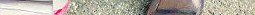
\includegraphics[width=\paperwidth]{footer.jpg}}
    \end{center}
 
\end{titlepage}
\ClearShipoutPicture

\begin{itemize}
   \item https://www.nouvelobs.com/rue89/nos-vies-intimes/20180723.OBS0077/grave-ou-aigue-sombre-ou-claire-ce-que-le-genre-fait-a-notre-voix.html
   \item https://matheo.uliege.be/handle/2268.2/2191
   \item https://www.cairn.info/revue-langage-et-societe-2015-1-page-7.html
\end{itemize}

Problématique :\\
Comment le genre d'un.e locuteur.ice du français influe sur sa prosodie?

Déroulement session 1 vendredi 7/10
lecture de https://www.cairn.info/revue-langage-et-societe-2015-1-page-7.html
   \enquote{Les aspects novateurs concernant les dynamiques du changement linguistique (attrition, nivellement) ou les patterns de variation genrée ont été « redécouverts » tout récemment.}
   repère 34
   \enquote{thèses de doctorat, notamment celle de Fagyal (1995) sur le style vocal de Marguerite Duras selon les situations}
   repère 36
   \enquote{Concernant le français, le courant cognitif est surtout représenté par des études en acquisition (cf. Nardy, Chevrot et Barbu dans ce numéro) mais nous pouvons également mentionner la thèse d’Aubanel (2011) qui cherche à articuler expérimentalement étude de la variation phonétique diatopique, interaction conversationnelle, traitement automatique et « caractérisation des représentations mentales associées aux sons de la parole ». }
   TROP INTERESSANT, repère 38
établissement d'une problématique
 
 
\end{document}


Page de garde :

    nom de l'université ou logo,
    nom et code de l'UE,
    année universitaire,
    formation (licence  SDL  première  année et mineure de découverte)
    nom de l'enseignant et groupe de TD / ou SED
    votre  nom  et  prénom
    votre numéro d'étudiant
    titre = votre thématique
    sous-titre = votre problématique
    image illustrant la thématique

Deuxième page :

    table des matières
    introduction
